%Группа 5-1 Модуль 1 Занятие №1
\begin{listofex}
	\item Вычислить:
	\begin{enumcols}[itemcolumns=2]
		\item \exercise{4161}
		\item \exercise{4162}
		\item \exercise{4163}
		\item \exercise{4164}
	\end{enumcols}
	\item \exercise{4165}
\end{listofex}
\newpage
\title{Занятие №2}
\begin{listofex}
	\item \exercise{4166}
	\item \exercise{4167}
	\item \exercise{4168}
	\item \exercise{4169}
	\item \exercise{4170}
	\item \exercise{4171}
	\item \exercise{4172}
	\item \exercise{4173}
\end{listofex}
\newpage
\title{Домашняя работа №1}
\begin{listofex}
	\item \exercise{4174} 
	\item \exercise{4175}
	\item \exercise{4176}
	\item \exercise{4177}
	\item \exercise{4178}
\end{listofex}
\newpage
\title{Занятие №3}
\begin{listofex}
	\item Вычислите, используя распределительный закон:
	\begin{enumcols}[itemcolumns=2]
		\item \( 7\cdot13-7\cdot2 \)
		\item \( 37\cdot12+37\cdot88 \)
		\item \( 101\cdot17-17 \)
		\item \( 33\cdot11+11 \)
	\end{enumcols}
	\item Перепишите заполняя пропуски:
	\begin{enumcols}[itemcolumns=2]
		\item \( {\dots}\cdot(16+14)=7\cdot16+7\cdot14 \)
		\item \( 45\cdot({\dots}-{\dots})=45\cdot15-45\cdot13 \)
		\item \( 14\cdot(15+3)=14\cdot{\dots}+{\dots}\cdot3 \)
		\item \( 7\cdot({\dots}+14)=14\cdot{\dots}+{\dots}\cdot5 \)
	\end{enumcols}
	\item Вынести общий множитель за скобки и вычислить:
	\begin{enumcols}[itemcolumns=2]
		\item \( 61\cdot21+39\cdot21 \)
		\item \( 123\cdot11-22\cdot11 \)
		\item \( 37\cdot59+37\cdot41+63\cdot59+41\cdot63 \)
		\item \( 999\cdot55+55+257\cdot43+43\cdot43 \)
	\end{enumcols}
	\item В магазине «Спортмастер» цена футбольного мяча равна \( a \) рублей, а цена баскетбольного
	мяча \( b \) рублей. Какой смысл имеют следующие выражения:
	\begin{enumcols}[itemcolumns=5]
		\item \( a+b \)
		\item \( a-b \)
		\item \( 2\cdot a + 3\cdot b \)
		\item \( 7\cdot a - 2\cdot b \)
		\item \( 5000 - (a+b) \)
	\end{enumcols}
	\item В двух комнатах было \( 45 \) человек. Из первой вышли \( 9 \), а из второй --- \( 14 \), и людей в комнатах стало поровну. Сколько человек было в комнатах сначала?
	\item Сошлись два пастуха Иван и Пётр. Иван говорит Петру: «Отдай мне одну овцу,
	тогда у меня будет ровно вдвое больше овец, чем у тебя.» А Пётр ему отвечает: «Нет!
	Лучше ты мне отдай одну овцу, тогда у нас овец будет поровну». Сколько же было овец у
	каждого?
	\item Зная, что \( 25\cdot4=100 \), вычислите устно:
	\begin{enumcols}[itemcolumns=4]
		\item \( 16\cdot25 \)
		\item \( 25\cdot80 \)
		\item \( 52\cdot25 \)
		\item \( 25\cdot844 \)
	\end{enumcols}
	\item Зная, что \( 125\cdot8=1000 \), вычислите устно:
	\begin{enumcols}[itemcolumns=4]
		\item \( 125\cdot24 \)
		\item \( 125\cdot80 \)
		\item \( 64\cdot125 \)
		\item \( 248\cdot125 \)
	\end{enumcols}
\end{listofex}
\newpage
\title{Занятие №4}
\begin{listofex}
	\item Вычислите, используя распределительный закон:
	\begin{enumcols}[itemcolumns=2]
		\item \( 18\cdot9-18\cdot7 \)
		\item \( 37\cdot12-37\cdot2 \)
		\item \( 99\cdot15+15 \)
		\item \( 201\cdot44-44 \)
	\end{enumcols}
	\item Перепишите заполняя пропуски:
	\begin{enumcols}[itemcolumns=2]
		\item \( {\dots}\cdot(13-2)=8\cdot2-8\cdot2 \)
		\item \( 16\cdot({\dots}-\dots)=16\cdot3-16 \)
		\item \( 2\cdot(6+17)=2\cdot{\dots}+{\dots}\cdot2 \)
		\item \( 7\cdot({\dots}+1)=15\cdot{\dots}+{\dots} \)
	\end{enumcols}
	\item Вынести общий множитель за скобки и вычислить:
	\begin{enumcols}[itemcolumns=3]
		\item \( 47\cdot42+42\cdot153 \)
		\item \( 35\cdot36-35\cdot34 \)
		\item \( 7\cdot55+7\cdot45+3\cdot45+3\cdot55 \)
	\end{enumcols}
	\item В двух комнатах было \( 64 \) человек. Из первой вышли \( 12 \), а из второй --- \( 15 \), и людей в комнатах стало поровну. Сколько человек было в комнатах сначала?
	\item Сошлись два пастуха Иван и Пётр. Иван говорит Петру: «Отдай мне две овцы,
	тогда у меня будет ровно вдвое больше овец, чем у тебя.» А Пётр ему отвечает: «Нет!
	Лучше ты мне отдай две овцы, тогда у нас овец будет поровну». Сколько же было овец у
	каждого?
	\item Придумайте (и запишите в тетради!) задачи, математической моделью которых могут
	являться следующие числовые и буквенные выражения:
	\begin{enumcols}[itemcolumns=3]
		\item \( 5\cdot15-2 \)
		\item \( 4000:2+2000:5 \)
		\item \( a+(3+b):c \)
	\end{enumcols}
	\item Зная, что \( 25\cdot4=100 \), вычислите устно:
	\begin{enumcols}[itemcolumns=4]
		\item \( 8\cdot25 \)
		\item \( 25\cdot40 \)
		\item \( 64\cdot25 \)
		\item \( 25\cdot420 \)
	\end{enumcols}
	\item Зная, что \( 125\cdot8=1000 \), вычислите устно:
	\begin{enumcols}[itemcolumns=4]
		\item \( 125\cdot16 \)
		\item \( 125\cdot800 \)
		\item \( 160\cdot125 \)
		\item \( 88\cdot125 \)
	\end{enumcols}
\end{listofex}
\newpage
\title{Домашняя работа №2}
\begin{listofex}
	\item Вычислите, используя распределительный закон:
	\begin{enumcols}[itemcolumns=2]
		\item \( 5\cdot23-5\cdot8 \)
		\item \( 54\cdot36-54\cdot6 \)
		\item \( 199\cdot87+87 \)
		\item \( 501\cdot70-70 \)
	\end{enumcols}
	\item Перепишите заполняя пропуски:
	\begin{enumcols}[itemcolumns=2]
		\item \( {\dots}\cdot(27+3)=4\cdot27-4\cdot3 \)
		\item \( 11\cdot({\dots}+{\dots})=11\cdot13+15 \)
		\item \( 33\cdot(4+11)=33\cdot{\dots}+33\cdot{\dots} \)
		\item \( 12\cdot({\dots}-1)=10\cdot{\dots}-{\dots} \)
	\end{enumcols}
	\item Вынести общий множитель за скобки и вычислить:
	\begin{enumcols}[itemcolumns=3]
		\item \( 51\cdot43+12\cdot43 \)
		\item \( 51\cdot81-39\cdot81 \)
		\item \( 8\cdot2+2\cdot92+8\cdot98+2\cdot8 \)
	\end{enumcols}
	\item Вычислите рациональным образом:
	\begin{enumcols}[itemcolumns=2]
		\item \( (5486+3578)+1422 \)
		\item \( (357+768+589)+(332+211+643) \)
	\end{enumcols}
	\item У Максима и Кости коллекции редких монет. Максим говорит Косте: «Отдай мне три монеты, тогда у меня будет в три раза больше
	монет, чем у тебя.» А Костя отвечает: «Нет! Лучше отдай ты мне три монеты, тогда у нас будет монет поровну. Сколько монет у каждого?
	\item Придумайте (и запишите в тетради!) задачи, математической моделью которых могут
	являться следующие числовые и буквенные выражения:
	\begin{enumcols}[itemcolumns=3]
		\item \( 7\cdot18+23 \)
		\item \( 2500 - 3\cdot x \)
		\item \( (a+b):7+c \)
	\end{enumcols}
\end{listofex}
\newpage
\title{Занятие №5}
\begin{listofex}
	\item Сформулировать признаки делимости на \( 2 \); \( 3 \); \( 5 \); \( 9 \); \( 10 \).
	\item Воспользуйтесь признаками делимости из предыдущего задания и определите, на что делятся данные числа:
	\begin{enumcols}[itemcolumns=5]
		\item \( 368 \)
		\item \( 585 \)
		\item \( 2450 \)
		\item \( 12321 \)
		\item \( 303030 \)
	\end{enumcols}
	\item \textbf{Свойства делимости:}
	\begin{enumcols}[itemcolumns=1]
		\item Если один из множителей делится на некоторое число, то и произведение делится на это число.
		\item Если первое число делится на второе, а второе делится на третье, то первое число делится на третье.
		\item Если каждое из двух чисел делится на некоторое число, то их сумма или разность делятся на это число.
		\item Если одно из двух чисел делится на некоторое число, а другое на него не делится, то их сумма или разность не делится на это число.
	\end{enumcols}
	\item Объясните, не производя вычислений, почему следующие произведения делятся на \( 12 \)? Каким свойством вы в это случае пользуетесь?
	\begin{enumcols}[itemcolumns=4]
		\item \( 12\cdot47 \)
		\item \( 24\cdot17 \)
		\item \( 120\cdot51 \)
		\item \( 27\cdot8 \)
	\end{enumcols}
	\item Запишите чиста \( 24,\;42,\;36,\;72,\;75 \) в виде произведения и покажите, что
	\begin{enumcols}[itemcolumns=3]
		\item \( 24 \) делится на \( 2 \)
		\item \( 36 \) делится на \( 6 \)
		\item \( 75 \) делится на \( 5 \)
		\item \( 42 \) делится на \( 21 \)
		\item \( 72 \) делится на \( 9 \)
		\item \( 75 \) делится на \( 25 \)
	\end{enumcols}
	\item Объясните, почему:
	\begin{enumcols}[itemcolumns=2]
		\item сумма \( 45+36 \) делится на \( 9 \)
		\item сумма \( 99+88 \) делится на \( 11 \)
		\item сумма \( 13\cdot2+13\cdot7\) делится на \( 13 \)
	\end{enumcols}
	\item Доказать, что:
	\begin{enumcols}[itemcolumns=1]
		\item произведение четного числа и любого натурального числа является четным числом;
		\item сумма двух четных чисел является четным числом;
		\item сумма двух нечетных чисел является четным числом;
		\item сумма четного и нечетного числа является нечетным числом.
	\end{enumcols}
	\item Какую цифру нужно поставить вместо звездочки, чтобы полученное число:
	\begin{enumcols}[itemcolumns=3]
		\item \( 2\:* \) делилось на \( 2 \);
		\item \( 43\:* \) делилось на \( 3 \);
		\item \( 4\:* \) делилось на \( 9 \);
		\item \( 23\:* \) делилось на \( 10 \);
		\item \( 123\:* \) делилось на \( 5 \);
		\item \( 24*0 \) делилось на \( 9 \);
		\item \( 2*22 \) делилось на \( 9 \);
		\item \( 1*4\:* \) делилось на \( 2 \) и \( 3 \);
		\item \( 4*5\:* \) делилось на \( 9 \) и \( 5 \).
	\end{enumcols}
	%\item Что такое простые числа? Что такое составные числа?
\end{listofex}
%\newpage
%\title{Занятие №6}
%\begin{listofex}
%	\item 1
%\end{listofex}
%\newpage
%\title{Домашняя работа №3}
%\begin{listofex}
%	\item 1
%\end{listofex}
%\newpage
\title{Занятие №7}
\begin{listofex}
	\item Разложить на простые множители:
	\begin{enumcols}[itemcolumns=5]
		\item \( 50 \)
		\item \( 44 \)
		\item \( 76 \)
		\item \( 420 \)
		\item \( 198 \)
		\item \( 220 \)
		\item \( 132 \)
		\item \( 384 \)
	\end{enumcols}
	\item Найти все делители числа:
	\begin{enumcols}[itemcolumns=5]
		\item \( 18 \)
		\item \( 55 \)
		\item \( 57 \)
		\item \( 102 \)
		\item \( 96 \)
	\end{enumcols}
	\item Вычислить:
	\begin{enumcols}[itemcolumns=6]
		\item \( 5^2 \)
		\item \( 3^3 \)
		\item \( 13^2 \)
		\item \( 300^2 \)
		\item \( 20^3 \)
		\item \( 110^2 \)
	\end{enumcols}
	\item Вычислить:
	\begin{enumcols}[itemcolumns=2]
		\item \( 3^2\cdot18 \)
		\item \( 2^5+3^4\)
		\item \( 17^2-209 \)
		\item \( (7^3-4^3):(7-4) \)
		\item \( 42^2:28+35\cdot10^2 \)
	\end{enumcols}
	\item Представьте число в виде квадрата или куба другого числа:
	\begin{enumcols}[itemcolumns=2]
		\item \( 9 \)
		\item \( 27 \)
		\item \( 100 \)
		\item \( 1000 \)
		\item \( 225 \)
		\item \( 1600 \)
	\end{enumcols}
	\item Замените буквы цифрами так, чтобы равенство оказалось верным
	\begin{enumcols}[itemcolumns=2]
		\item AB + BC + ABC = BCB
		\item ЛИК \( \cdot \) ЛИК = БУБЛИК
	\end{enumcols}
\end{listofex}
%\newpage
%\title{Занятие №8}
%\begin{listofex}
%	\item 1
%\end{listofex}
%\newpage
%\title{Домашняя работа №4}
%\begin{listofex}
%	\item 1
%\end{listofex}
\newpage
\title{Проверочная работа}
\begin{listofex}
	\item Вычислить:
	\begin{enumcols}[itemcolumns=1]
		\item \exercise{4161}
		\item \exercise{4164}
	\end{enumcols}
	\item Вычислите, используя распределительный закон (кроме ответа, распишите то, как вы применяете этот закон):
	\begin{enumcols}[itemcolumns=2]
		\item \( 6\cdot13-6\cdot2 \)
		\item \( 101\cdot20-20 \)
	\end{enumcols}
	\item Перепишите заполняя пропуски:
	\begin{enumcols}[itemcolumns=2]
		\item \( {\dots}\cdot(16+14)=7\cdot16+7\cdot14 \)
		\item \( 45\cdot({\dots}-{\dots})=45\cdot15-45\cdot13 \)
	\end{enumcols}
	\item В двух комнатах было \( 45 \) человек. Из первой вышли \( 9 \), а из второй --- \( 14 \), и людей в комнатах стало поровну. Сколько человек было в комнатах сначала?
	\item Выпишите числа, которые делятся на \( 2 \) и числа, которые делятся на \( 3 \) (числа могут входить в обе группы):
	\begin{enumcols}[itemcolumns=6]
		\item \( 368 \)
		\item \( 579 \)
		\item \( 1122 \)
		\item \( 972 \)
		\item \( 21346\)
		\item \( 101010 \)
	\end{enumcols}
	\item Какие из следующих произведений делятся на \( 14 \)? Объясните почему?
	\begin{enumcols}[itemcolumns=4]
		\item \( 14\cdot45 \)
		\item \( 12\cdot3 \)
		\item \( 17\cdot28 \)
		\item \( 21\cdot10 \)
	\end{enumcols}
	\item Города \( A \) и \( B \) расположены на одном шоссе на расстоянии 90 км. Из города \( B \) в
	направлении города \( A \) выехал велосипедист со скоростью \( 15 \) км/ч.
	\begin{enumcols}[itemcolumns=1]
		\item[А)] Через какое время после начала движения велосипедист приедет в город \( A \) ?
		\item[Б)] Через какое время после начала движения велосипедист окажется ровно посередине между
		городами \( A \) и \( B \) ?
		\item[В)] На каком расстоянии от города \( A \) окажется велосипедист через 8 часов после начала
		движения?
	\end{enumcols}
\end{listofex}
\newpage
\title{Консультация}
\begin{listofex}
	\item На некоторой книжной полке книги стоят в один ряд. Самая большая и самая маленькая книги обе стоят вплотную к самой старой книге. Слева от самой большой
	книги стоит 20 книг, а справа от самой маленькой – 17 книг. Сколько книг может
	стоять на этой полке? Укажите в ответе наименьшее возможное число книг!
	\item В кружки на рисунке требуется вписать числа 1, 2, 3, 4 или 5 так, чтобы в кружках,
	соединённых линией, оказались разные числа (иными словами, не должно быть двух
	кружков, соединённых линией, в которых написаны одинаковые числа). Некоторые
	кружки уже заполнены. Остальные – пока нет. Заполните их (у себя в тетради или в
	уме). Какое число будет в кружочке, закрашенном более тёмным цветом? (Обратите
	внимание, что все кружочки на картинке должны быть заполнены числами (каждый
	– одним из чисел 1, 2, 3, 4, 5). А в поле для ответа нужно вписать только то число,
	которое должно быть в более тёмном кружочке. Если есть несколько подходящих
	чисел, впишите в ответ самое большое из них.)
	\begin{center}
		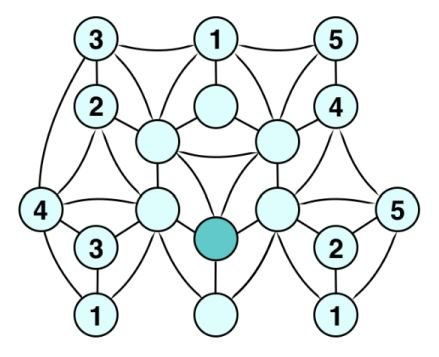
\includegraphics[width=0.5\linewidth]{123.jpg}
	\end{center}
	\item Из карточек с цифрами 1, 2, 3, 4, 5, 6 котенок Гав составляет три двузначных числа.
	Председатель Общества симпатичных котят выбирает самое большое из чисел, составленных котенком Гав, после чего котенок должен заплатить членский взнос, равный
	этому числу. Подумайте, как котенку Гав составить числа так, чтобы заплатить как
	можно меньше. Укажите в ответе самую меньшую сумму, которую котенку придется заплатить.
	\item На шахматном турнире Остап Бендер должен сыграть 15 партий. В какой-то момент во время турнира Остап отметил, что на данный момент он выиграл ровно треть
	сыгранных партий, а проиграл ровно четверть сыгранных партий (остальные уже сыгранные партии закончились вничью). Сколько еще партий осталось сыграть Остапу?
	\item Решить ребус: СИНИЦА \( + \) СИНИЦА \( = \) ПТИЧКИ
\end{listofex}